\textbf{Монолитная BMS ---} разработаны для определенных конфигураций блоков. Они предлагают простоту и экономичность. 
Немодульные решения BMS предполагается использовать там, где размер и конфигурация аккумуляторной батареи остаются постоянными. 
Они устраняют необходимость в дополнительной проводке и обеспечивают простое решение. 
Не модульная система часто задрудняет обслуживание батареи, в частности замена отдельных неисправных ячеек.

\textbf{Модульная система управления ---} состоит из нескольких блоков, которые можно легко соединять или отключать для реализации различных конфигураций батарей. 
Это обеспечивает гибкость при создании батареи, масштабируемость, простоту обслуживания.
Однако модульные решения BMS могут иметь большее кол-во проводки и усложнение элементов корпуса, что может отразится на цене и весе батареи.

Примером модульной системы является проект с отрытым исходным кодом --- Smart BMS (см. \figurename\ref{fig:smart_bms})
\begin{figure}[h]
	\centering
	\begin{minipage}{0.45\linewidth}
		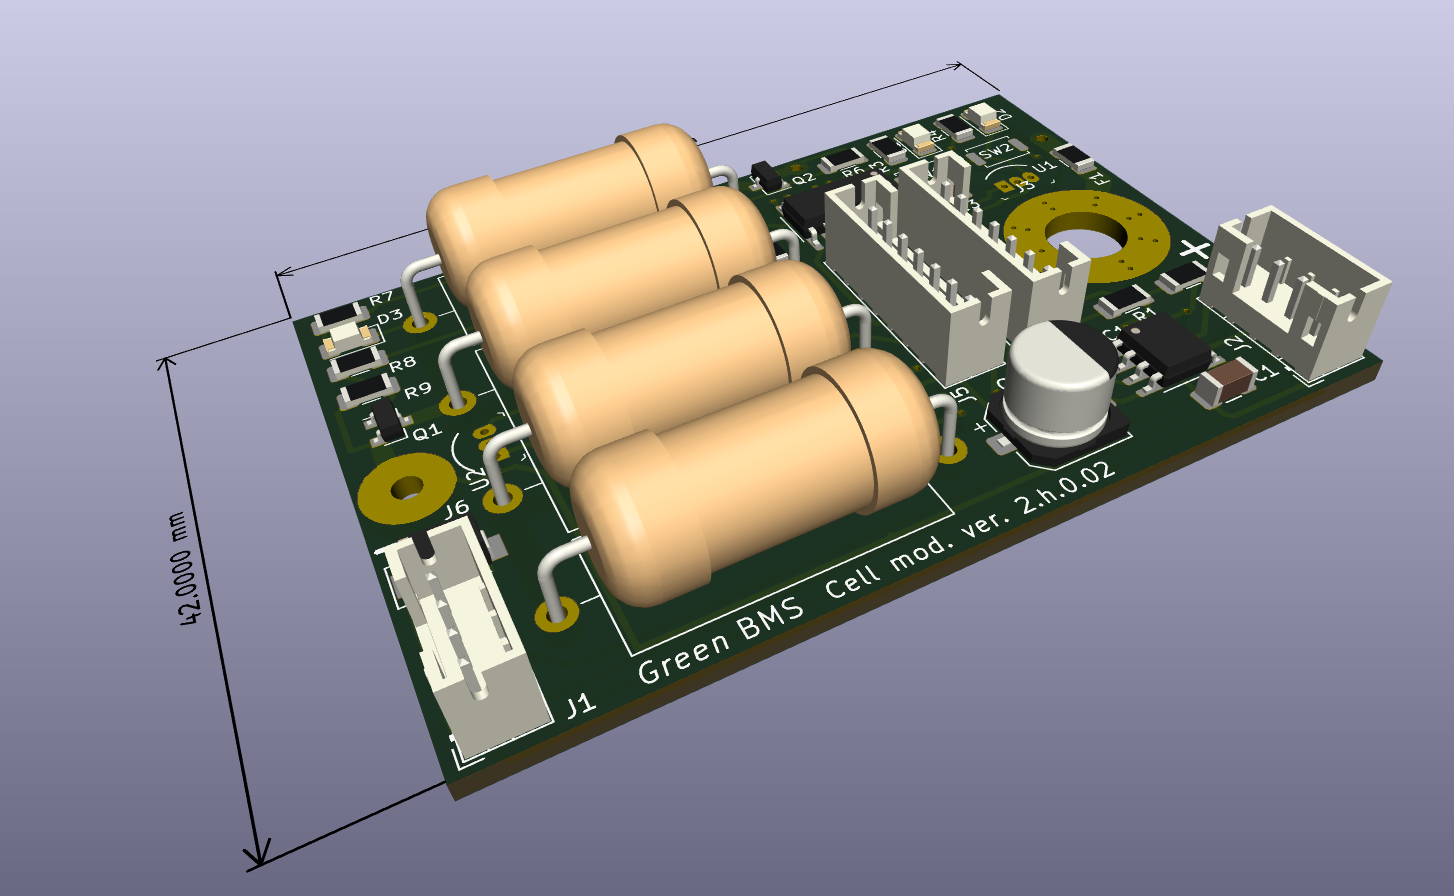
\includegraphics[width=\linewidth]{img/smart_bms_cell_1.png}
		\subcaption{Плата-slave(вид сбоку)}
		% \label{fig:smart_bms_slave_1}
	\end{minipage}
	\begin{minipage}{0.45\linewidth}
	    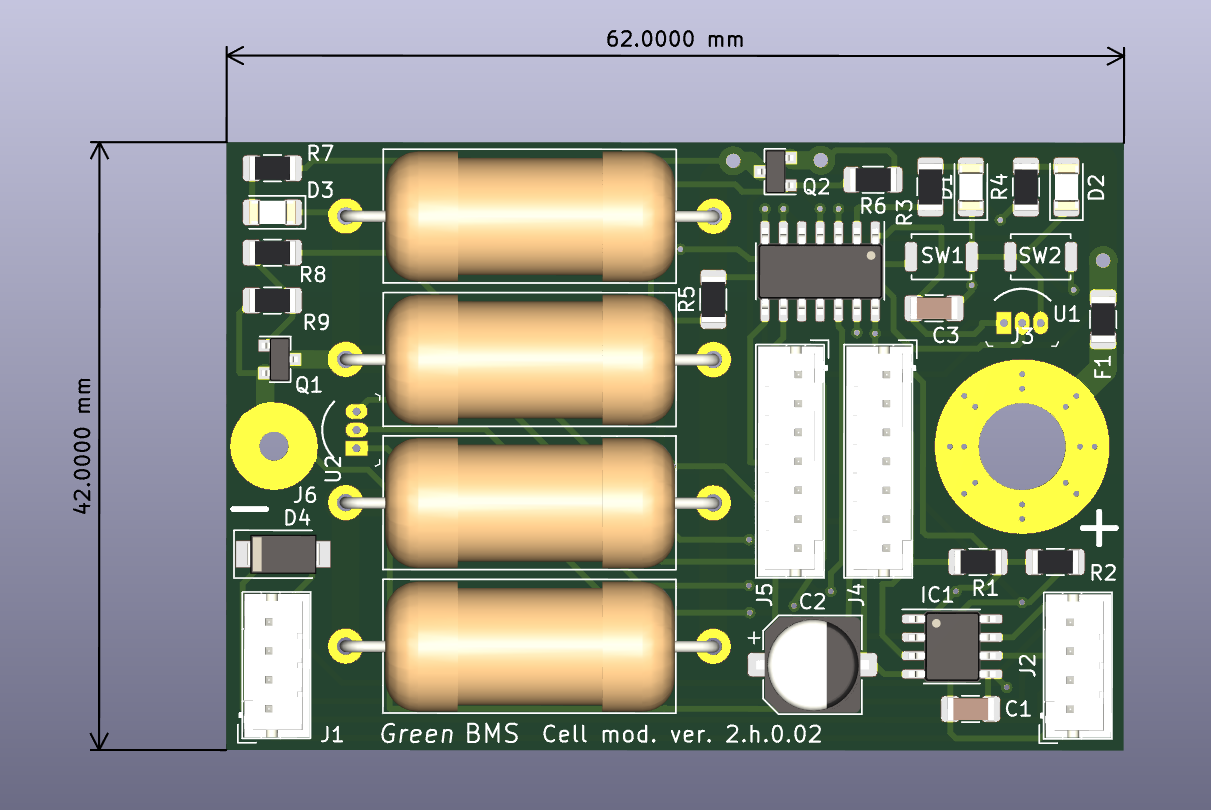
\includegraphics[width=\linewidth]{img/smart_bms_cell_2.png}
	    \subcaption{Плата-slave(вид сверху)}
	    % \label{fig:smart_bms_slave_2}
        \end{minipage} \\	
	\begin{minipage}{0.45\linewidth}
	    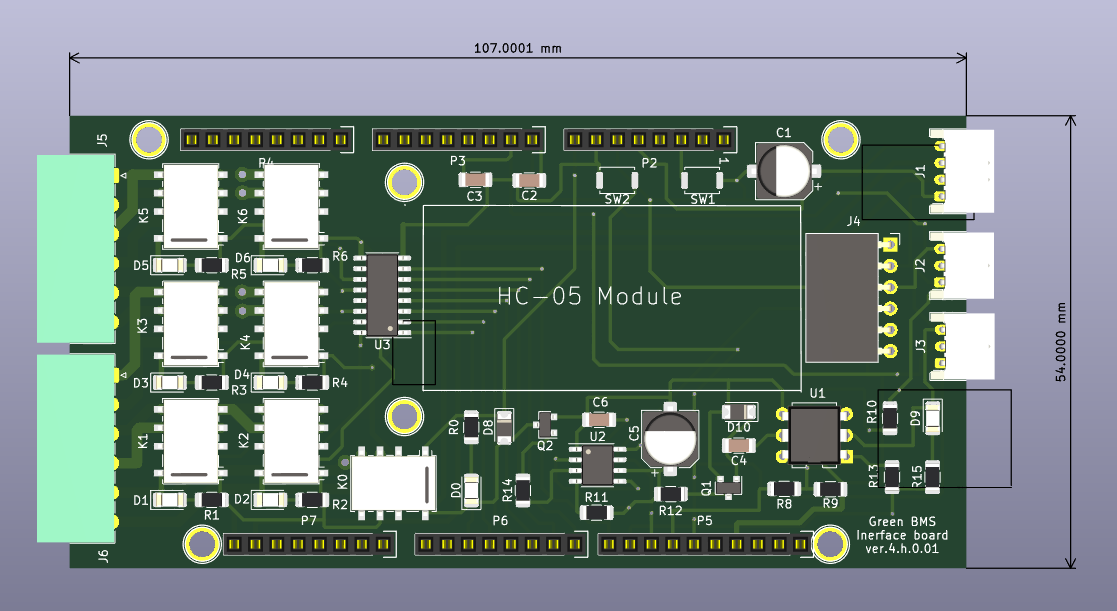
\includegraphics[width=\linewidth]{img/smart_bms_ctrl.png}
	    \subcaption{Плата-мастер}
	    % \label{fig:smart_bms_master}
    \end{minipage}
\caption{Составляющие Smart BMS}
\label{fig:smart_bms}
\end{figure}